% Copyright (C) 2011 by Thomas Moulard, LAAS-CNRS.
%
% Humanoids'11 workshop presentation


\documentclass[hyperref={pdfpagelabels=false}]{beamer}

%%%%%%%%%%%%%%%%%%%%%%%%%%%%%%%%%%%%%%%%%%%%%%%%%%%%%%%%%%%%%%%%%%%%%%%%%%%%%%%%
%% LaTeX and Beamer setup.                                                    %%
%%%%%%%%%%%%%%%%%%%%%%%%%%%%%%%%%%%%%%%%%%%%%%%%%%%%%%%%%%%%%%%%%%%%%%%%%%%%%%%%

\usepackage{lmodern}

\usepackage{beamerthemesplit}
\usepackage{multimedia}

\usepackage{amsmath}
\usepackage{amsfonts}
\usepackage{array}

\usepackage{url}

\usepackage{tikz, pgfplots}

\usetikzlibrary{patterns}
%\usetikzlibrary{external}
%\tikzexternalize

% Use tuned Warsaw theme.
\mode<presentation>
{
  \usetheme{Madrid}
  \usecolortheme{whale}
  \setbeamercolor{uppercol}{fg=white,bg=blue!40}
  \setbeamercolor{lowercol}{fg=black,bg=blue!15}
  \beamertemplateshadingbackground{blue!5}{blue!20}
  \beamertemplatenavigationsymbolsempty
}

% Allow Metapost file inclusion.
\ifx\pdftexversion\undefined
 \usepackage{graphicx}
\else
 \usepackage{graphicx}
 \DeclareGraphicsRule{*}{mps}{*}{}
\fi

% Common packages.
\usepackage[english]{babel}
\usepackage{times}

\usepackage{tikz}

\usepackage{amsfonts}
\usepackage{amssymb}
\usepackage[footnote]{fixme}

% Tune bibliography style.
\usepackage[style=authortitle-icomp,natbib=true,sortcites=true,block=space]{biblatex}
\bibliography{11humanoids-tmoulard-slides}

% Get rid of navigation symbols.
\setbeamertemplate{navigation symbols}{}

%%%%%%%%%%%%%%%%%%%%%%%%%%%%%%%%%%%%%%%%%%%%%%%%%%%%%%%%%%%%%%%%%%%%%%%%%%%%%%%%
%% Meta-information.                                                          %%
%%%%%%%%%%%%%%%%%%%%%%%%%%%%%%%%%%%%%%%%%%%%%%%%%%%%%%%%%%%%%%%%%%%%%%%%%%%%%%%%
\title[Trajectory Following for Legged Robots]
{Trajectory Following for Legged Robots}

\author[Moulard \and Lamiraux \and Stasse]{T.~Moulard \and
  F.~Lamiraux \and
  O.~Stasse\texorpdfstring{\\
  \small{\texttt{thomas.moulard@laas.fr}}}{}}

\institute[LAAS]
{
  LAAS-CNRS, Universit\'e de Toulouse\\
  7, avenue du Colonel Roche\\
  31077 Toulouse cedex 4, France}

\date{October 2011}

\subject{Control loop aimed at precise, closed-loop, trajectory
  following for legged robots.}

% Add a table of content between each section.
\AtBeginSubsection[]
{
  \begin{frame}<beamer>{Outline}
    \tableofcontents[currentsection,currentsubsection]
  \end{frame}
}


%%%%%%%%%%%%%%%%%%%%%%%%%%%%%%%%%%%%%%%%%%%%%%%%%%%%%%%%%%%%%%%%%%%%%%%%%%%%%%%%
%% Document.                                                                  %%
%%%%%%%%%%%%%%%%%%%%%%%%%%%%%%%%%%%%%%%%%%%%%%%%%%%%%%%%%%%%%%%%%%%%%%%%%%%%%%%%
\begin{document}

\begin{frame}
  \titlepage
\end{frame}

\begin{frame}{Outline}
  \tableofcontents[pausesections]
\end{frame}

\section{Problem statement}

\begin{frame}{From motion planning\ldots}
  \begin{center}
    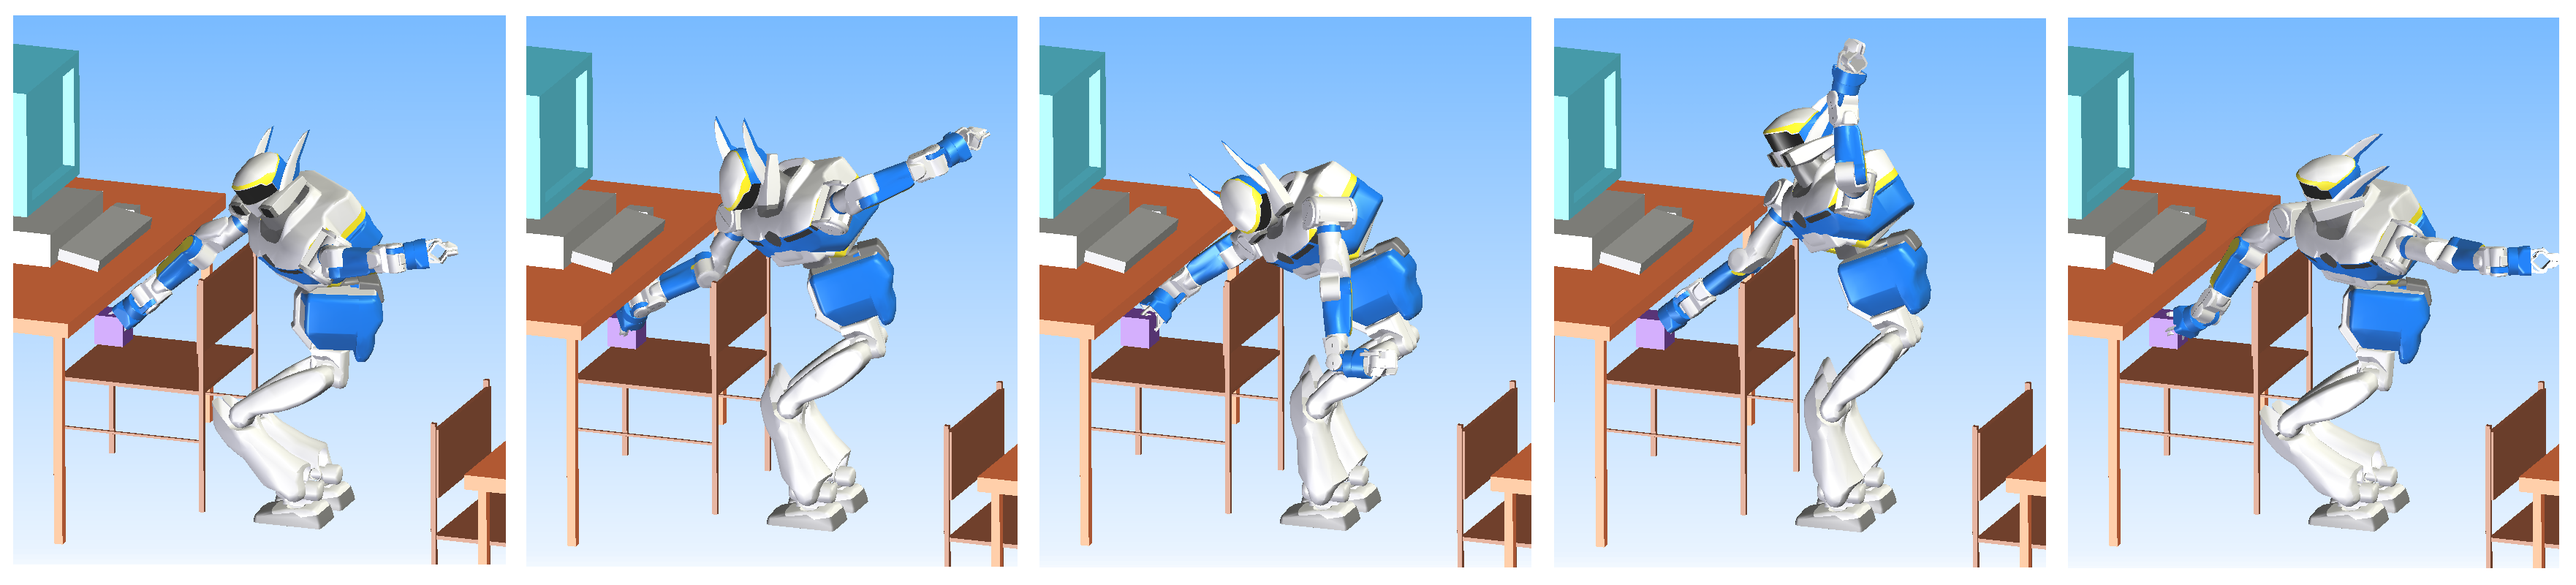
\includegraphics[width=0.99\linewidth]{fig/goal-generation.png}\\
    \vspace{0.5cm}
    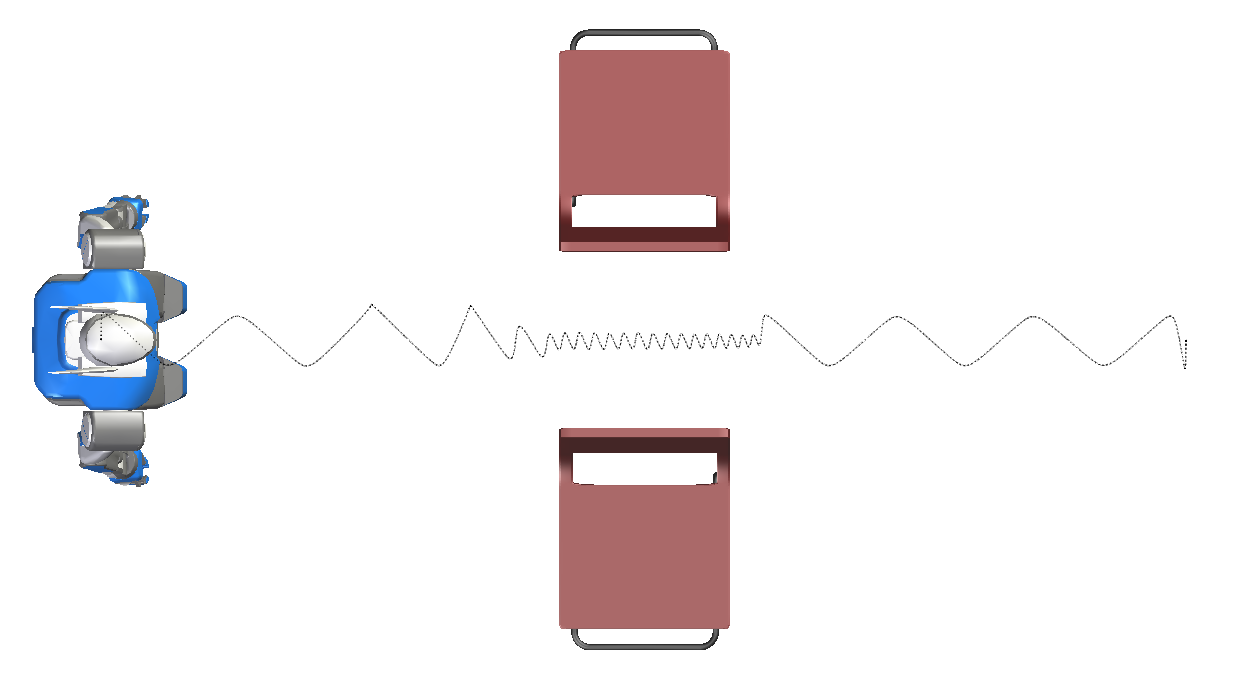
\includegraphics[width=0.5\linewidth]{fig/waist-trajectory.png}
  \end{center}
\end{frame}

\begin{frame}{\ldots to movement execution}
  \begin{center}
    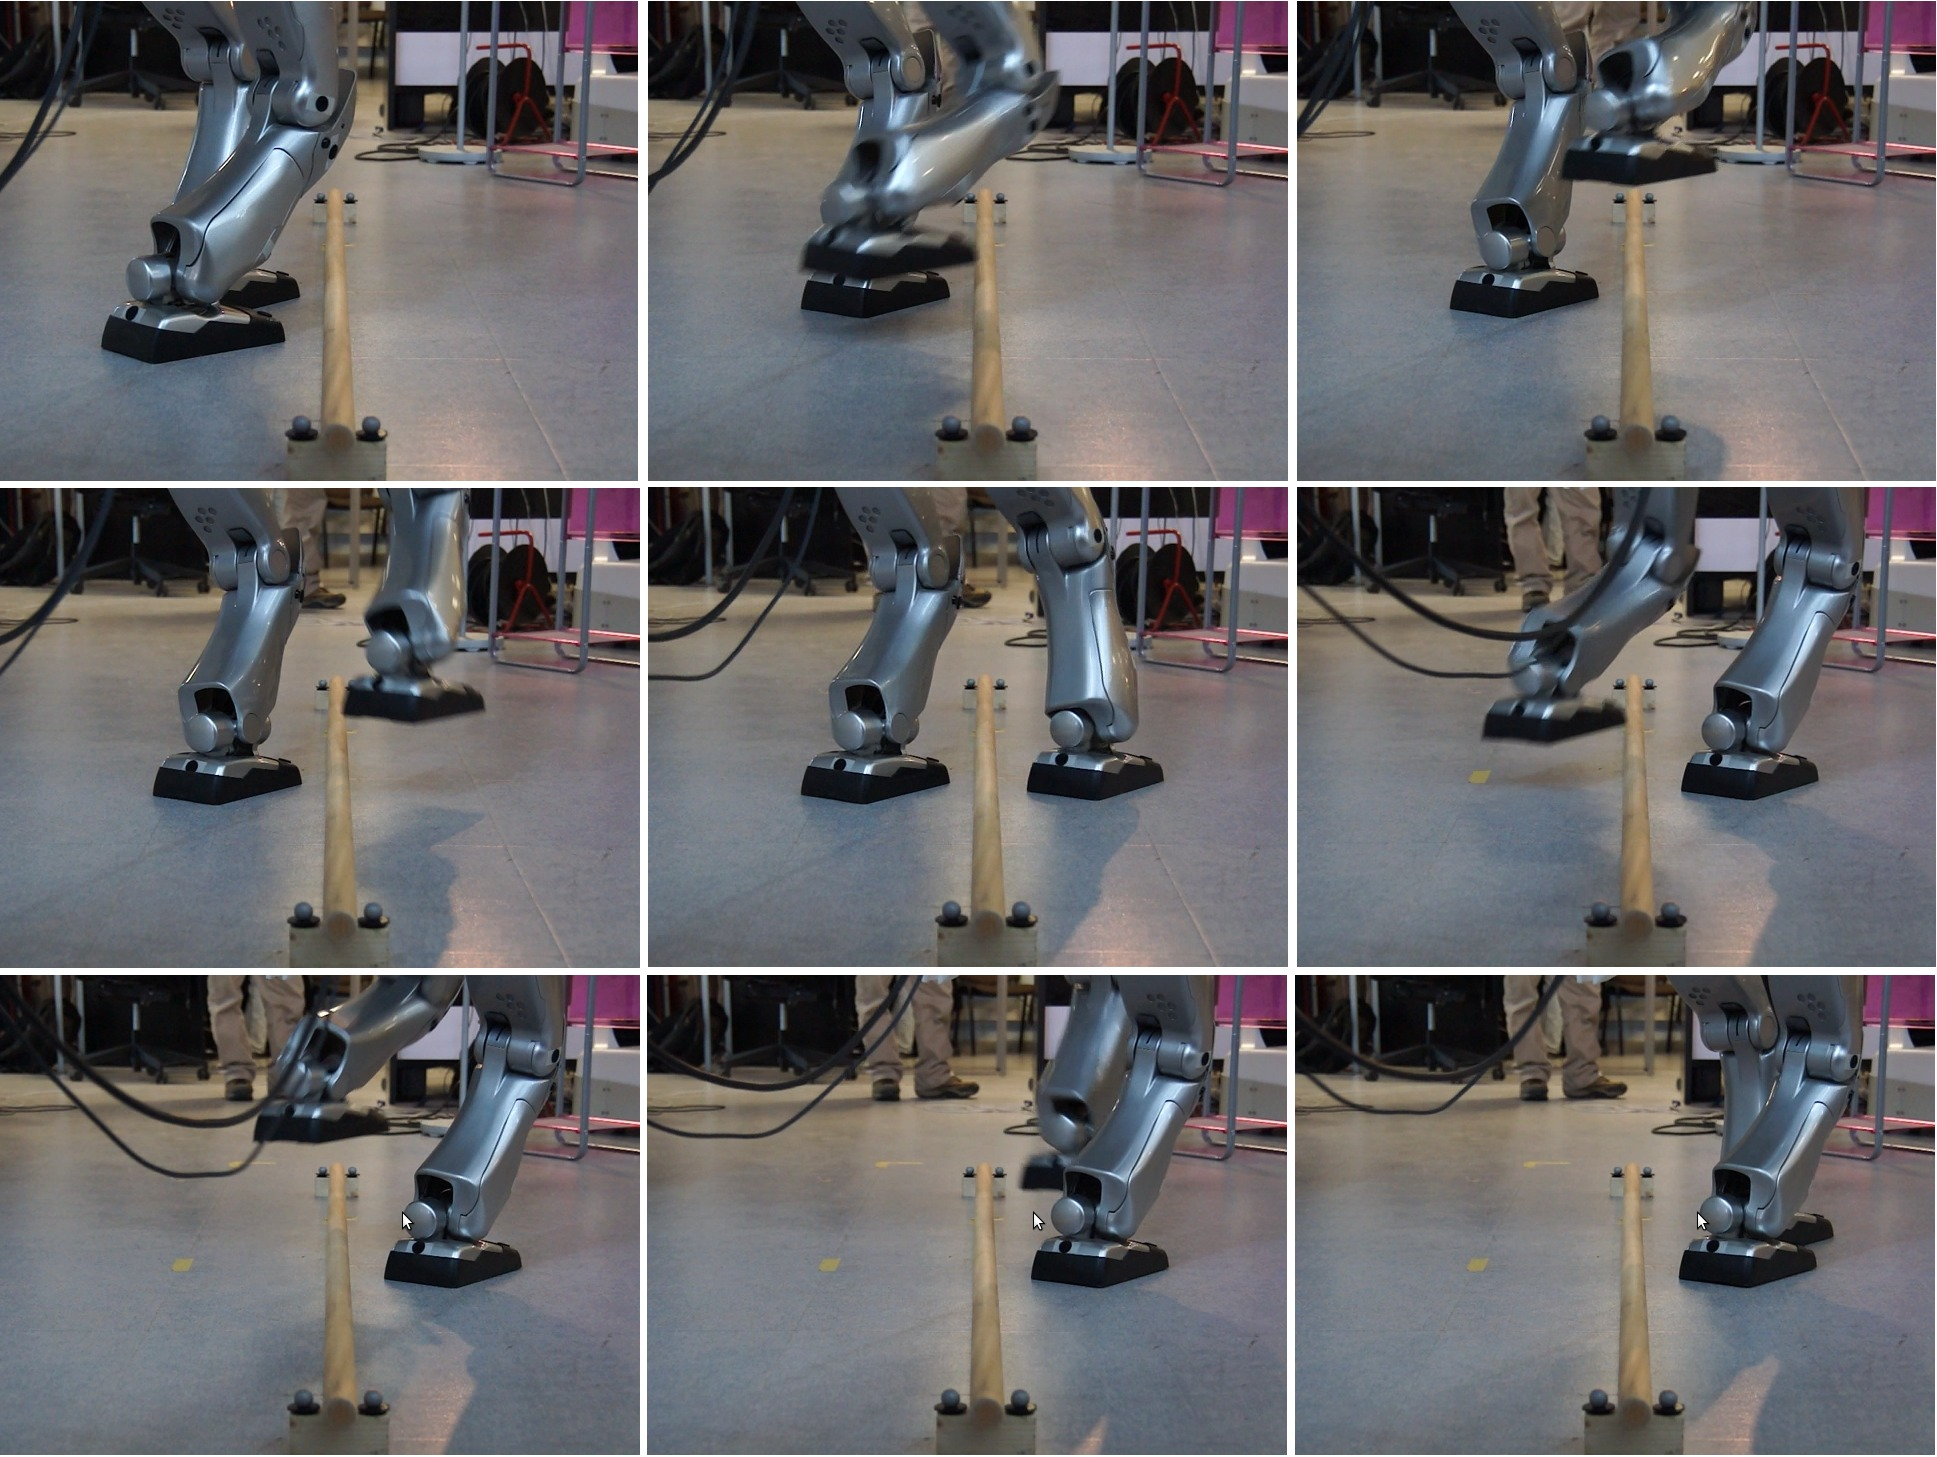
\includegraphics[height=7.5cm]{fig/over.jpg}
  \end{center}
\end{frame}

\begin{frame}{Why is it difficult?}
  \begin{itemize}
    \item Environment model errors.
    \item Significant walking drift (about $1\text{cm}$ per step).
    \item Computationally intensive to recompute the movement.

    \item Cannot apply mobile robotics strategies:
      \begin{itemize}
        \item Waist is locally controllable.
        \item Foot positions cannot be corrected simultaneously.
      \end{itemize}
  \end{itemize}

  \emph{These problems create a serious gap between what is feasible
    in simulation and what can be executed on the robot.}\\
  {
    \footnotesize
    \cite{11humanoids.baudouin}
  }
\end{frame}

\begin{frame}{Our motivation}
  \movie[showcontrols]{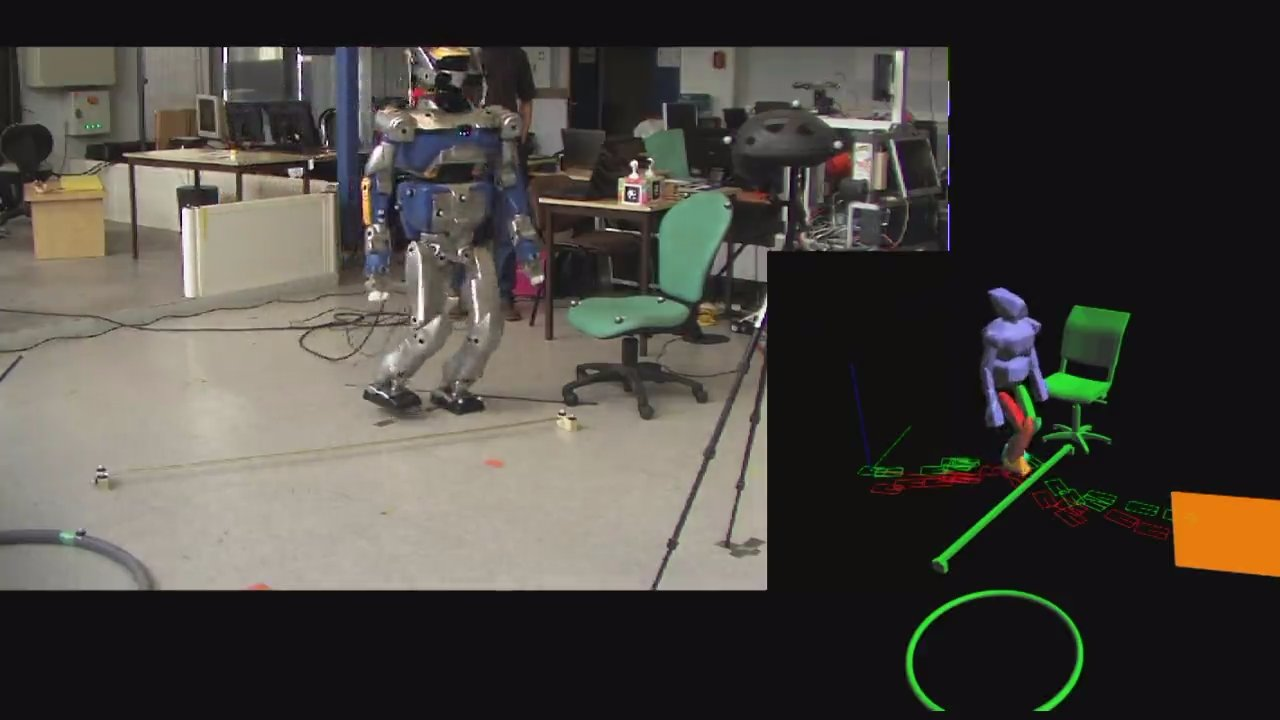
\includegraphics[width=\linewidth]{fig/lbaudouin.jpg}}{vid/humanoids11-lbaudouin.avi}
\end{frame}

\begin{frame}{What's next?}

  \begin{block}{Previous work}
    Previous work usually focused on ensuring robot balance when a
    perturbation occurs and not on following the plan as closely as
    possible.\\

    \footnotesize
    \cite{07icra.morisawa}
  \end{block}

  \begin{block}{Goal}
    \begin{itemize}
    \item Localize the robot.
    \item Online modification of the robot whole-body movement to
      cancel the drift with a control scheme \emph{suited} for
      humanoid robots.
    \end{itemize}
  \end{block}


\end{frame}


\section{Proposed closed-loop control scheme}

\begin{frame}{Closed-loop trajectory control scheme}

  \begin{center}
    \tikzstyle{state}=[rectangle,
      fill=blue!20,
      inner sep=0.2cm,
      rounded corners=2mm]

    \begin{tikzpicture}[>=latex]

      \draw (-1,-2) node [state] (ctrl) {Control framework};

      \draw (-1,0) node [state] (corr) {Trajectories Correction};
      \draw (-1,1.5) node [state] (gen) {Trajectories Generation};
      
      \draw (4,0) node (loc) [state] {Localization};

      \draw[-,style=dashed] (2,-3) -- (2,3);

      \draw<3->[->] (loc.west) -- (corr.east) node [at start,left,font=\tiny,yshift=0.2cm] {$\hat{\mathbf{x}}_t \in \text{SE}(2)$};

      \draw<1-2> (loc.west) node [at start,left,font=\tiny,yshift=0.2cm] {\phantom{$\hat{\mathbf{x}}_t \in \text{SE}(2)$}};


      \draw<2->[->] (gen.south) -- (corr.north) node [at start,left,font=\tiny,yshift=-0.2cm]
           {$(\gamma_{\text{left~foot}}(t), \gamma_{\text{right~foot}}(t), \gamma_{\text{com}}(t), \mathbf{x}(t)) \in \text{SE}(3)^3 \times \text{SE}(2)$};

      \draw<1> (gen.south) node [at start,left,font=\tiny,yshift=-0.2cm]
           {\phantom{$(\gamma_{\text{left~foot}}(t), \gamma_{\text{right~foot}}(t), \gamma_{\text{com}}(t), \mathbf{x}(t)) \in \text{SE}(3)^3 \times \text{SE}(2)$}};


      \draw<3->[->] (corr.south) -- (ctrl.north) node [at start,left,font=\tiny,yshift=-0.25cm]
           {$(\gamma'_{\text{left~foot}}(t), \gamma'_{\text{right~foot}}(t), \gamma'_{\text{com}}(t)) \in \text{SE}(3)^3$};

      \draw<1-2> (corr.south) node [at start,left,font=\tiny,yshift=-0.25cm]
           {\phantom{$(\gamma'_{\text{left~foot}}(t), \gamma'_{\text{right~foot}}(t), \gamma'_{\text{com}}(t)) \in \text{SE}(3)^3$}};

      \draw<4->[->] (ctrl.south) --++ (0,-1) node [at start,left,font=\tiny,yshift=-0.25cm]
           {$\dot{\mathbf{q}}_t \in \mathbb{R}^n$};

      \draw<1-3> (-1,-3) node [at start,left,font=\tiny,yshift=-0.25cm]
           {\phantom{$\dot{\mathbf{q}}_t \in \mathbb{R}^n$}};

      \draw[<-] (gen.north) --++ (0,1) node [left,font=\tiny,yshift=-0.25cm]
           {footsteps $\mathbf{S} \in \text{SE}(2)^{\text{nsteps}}$};



    \end{tikzpicture}
  \end{center}
\end{frame}

\begin{frame}{Correction temporal synchronization}
\begin{figure}[ht!]
  \begin{center}
    \vspace{-1.5cm}
    \only<1->{
      \vspace{0.4cm}
    }
    \begin{tikzpicture}
      \begin{axis}[
          height=.8\textheight,
          width=.75\textwidth,
          grid=major,
          legend style={
            at={(0.5,-0.2)},
            anchor=north,
            legend columns=3,
            cells={anchor=west},
            font=\footnotesize,
            rounded corners=2pt,
            fill=blue!20
          },
          xlabel=time ($\mathrm{s}$),
          ylabel=$x$ position ($\mathrm{m}$),
          no markers
          ]

        \addplot[
          red,
          dashed,
        ] table[
          x expr=(\thisrowno{0}-0)*0.005
        ] {dat/feet_follower_feet-follower-com.dat};
        \addlegendentry{center of mass}

        \addplot[
          blue,
          dashed,
        ] table[
          x index=0,
          y index=4,
          x expr=(\thisrowno{0}-0)*0.005
        ] {dat/feet_follower_feet-follower-left-ankle.dat};
        \addlegendentry{left foot}

        \addplot[
          green,
          dashed,
        ] table[
          x index=0,
          y index=4,
          x expr=(\thisrowno{0}-0)*0.005
        ] {dat/feet_follower_feet-follower-right-ankle.dat};
        \addlegendentry{right foot}

        \only<7->{
        \addplot[
          red,
        ] table[
          x expr=(\thisrowno{0}-0)*0.005,
          y expr=\thisrowno{1}-0.
        ] {dat/feet_follower_correction-com.dat};
        \addlegendentry{center of mass (corr.)}
        }

        \only<6->{
        \addplot[
          blue,
        ] table[
          x index=0,
          y index=4,
          x expr=(\thisrowno{0}-0)*0.005,
          y expr=\thisrowno{4}-0.
        ] {dat/feet_follower_correction-left-ankle.dat};
        \addlegendentry{left foot (corr.)}
        }

        \only<5->{
        \addplot[
          green,
        ] table[
          x index=0,
          y index=4,
          x expr=(\thisrowno{0}-0)*0.005,
          y expr=\thisrowno{4}-0.
        ] {dat/feet_follower_correction-right-ankle.dat};
        \addlegendentry{right foot (corr.)}
        }
      \end{axis}

      \draw<2-> [
        thick,
        decoration={
          brace,
          raise=-1.05cm
        },
        font=\tiny,
        decorate
      ] (axis cs:2.1,6.35) -- (axis cs:4.1,6.35)
      node [pos=0.5,anchor=north,yshift=-0.55cm] {step 1};

      \draw<1>(axis cs:2.1,6.35)
      node [pos=0.5,anchor=north,yshift=-0.55cm] {\phantom{step 1}};

      \draw<3-> [
        thick,
        decoration={
          brace,
          raise=-1.05cm
        },
        font=\tiny,
        decorate
      ] (axis cs:5.1,6.35) -- (axis cs:7.1,6.35)
      node [pos=0.5,anchor=north,yshift=-0.55cm] {step 2};

      % error measure
      \draw<4->[<-]
      (1.3, 0.5) -- (1.3, 1.5)
      node [font=\tiny,anchor=north,yshift=0.3cm, line width=1.3]
      {error measure};

      \def\w{0.5}
      \def\h{0.75}
      \def\dx{8.}

      \def\dy{.5}
      % left step planned 1
      \filldraw[pattern=north east lines] (\dx + 0., \dy + 0.5)
      rectangle (\dx + 0. + \w, \dy + \h + 0.5);

      % left step planned 1 - drift
      \draw<4->[style=solid,color=red,line width=1.25] (\dx, \dy - 0.3 + 0.5)
      rectangle (\dx + \w, \dy + \h - 0.3 + 0.5);

      \filldraw[pattern=north east lines] (\dx + 1., \dy + 0.5)
      rectangle (\dx + 1. + \w, \dy + \h + 0.5);
      \draw<4->[style=solid,color=red,line width=1.25] (\dx + 1., \dy - 0.3 + 0.5)
      rectangle (\dx + \w + 1., \dy + \h - 0.3 + 0.5);


      % right step planned 1
      \filldraw[pattern=north east lines] (\dx + 1., \dy + 3.)
      rectangle (\dx + 1. + \w, \dy + \h + 3.)
      node [pos=0.5,anchor=north,font=\tiny,yshift=0.75cm] {step 1};

      % right step planned 1 - corrected
      \draw<4->[style=solid,color=red,line width=1.25] (\dx + 1., \dy + 3.-0.3)
      rectangle (\dx + 1. + \w, \dy + \h + 3. -0.3);


      \draw<5->[style=solid,color=green,line width=1.25] (\dx + 1., \dy + 3.)
      rectangle (\dx + 1. + \w, \dy + \h + 3.);

      \def\dy{3.}
      % left step planned 2
      \filldraw[pattern=north east lines] (\dx + 0., \dy + 0.5)
      rectangle (\dx + 0. + \w, \dy + \h + 0.5)
      node [pos=0.5,anchor=north,font=\tiny,yshift=0.75cm] {step 2};

      \draw<4->[style=solid,color=red,line width=1.25] (\dx, \dy + 0.5 -0.3)
      rectangle (\dx + \w, \dy + \h + 0.5 -0.3);

      % left step planned 2 - corrected
      \draw<6->[style=solid,color=green,line width=1.25] (\dx + 0., \dy + 0.5)
      rectangle (\dx + 0. + \w, \dy + \h + 0.5);


    \end{tikzpicture}
  \end{center}
\end{figure}
\end{frame}

\begin{frame}{1. Error estimation}

%  \begin{columns}
%    \begin{column}{0.5\textwidth}

      \begin{block}{Error computation}

        \begin{itemize}
        \item $\mathbf{x} \in \text{SE}(2)$ the planned position of the root body.
        \item $\hat{\mathbf{x}} \in \text{SE}(2)$ the root body position
          perceived by the localization system.
        \end{itemize}

        The error $\mathbf{\delta x} \in \text{SE}(2)$ is defined as:
        \begin{equation} \label{eq:errorpos}
          \mathbf{\delta x} = \mathbf{x} . \hat{\mathbf{x}}^{-1}
        \end{equation}
      \end{block}

%    \end{column}
%    \begin{column}{0.5\textwidth}

      \begin{figure}[ht!]
        \begin{center}
          \begin{tikzpicture}[x=.95\textwidth,y=2.5cm]
            \def\w{0.3}
            \def\h{0.35}

      \def\ws{0.05}
      \def\hs{0.2}

      \def\noisex{0.01}
      \def\noisey{0.3}

      \def\dx{0.}
      \def\dy{0.}

      \draw[pattern=dots,rounded corners]
      (0.,0.25+\dy) rectangle (0.+\w,0.25+\dy+\h);

      \draw[rotate=-10,rounded corners]
      (\noisex,0.25+\noisey + \dy) rectangle
      (\noisex+\w,0.25+\noisey+\dy+\h);

      \draw[smooth,rounded corners=1ex,<->,thick]
      (-0.02, 0.25+0.45) --
      (-0.03, 0.25+0.35) --
      (-0.02, 0.25+0.25)
      node[at start,left]
      {
        $\Delta r_z$
      };

      \draw[smooth,rounded corners=1ex,<->,thick]
      (-0.02, 0.25+0.) --
      (-0.02, 0.25+0.15)
      node[midway,left]
      {
        $\Delta x$
      };

      \draw[smooth,rounded corners=1ex,<->,thick]
      (0., 0.25-0.1) --
      (0.03, 0.25-0.1)
      node[midway,below]
      {
        $\Delta y$
      };

      \path node (txt1) at (0.11+\w,0.25+0.)
            [shape=rectangle,draw,color=black]
            {\color{black} $\mathbf{x}$};

      \path node (txt1) at (0.115+\w,0.25+0.3)
            [shape=rectangle,draw,color=black]
            {\color{black} $\mathbf{\hat{x}}$};
    \end{tikzpicture}
  \end{center}
\end{figure}
%\end{column}
%\end{columns}

\end{frame}

\begin{frame}{2a. Swing foot trajectory update}

  \begin{columns}[c]
    \begin{column}{0.5\textwidth}

      \begin{block}{Footstep update}
        \begin{itemize}
        \item A walk movement is a sequence of footsteps $S \in \text{SE}(2)^{\text{nsteps}}$.
        \item The remaining steps set is $S^{\text{future}}$.
        \item Remaining steps must be moved such that the next step
          will cancel the drift and reach the planned position.
        \end{itemize}

        \begin{equation} \label{eq:footstepmodif}
          \forall s \in S^{\text{future}}, s \gets \mathbf{\delta {x}} . s
        \end{equation}
      \end{block}

    \end{column}

    \begin{column}{0.5\textwidth}
      \vspace{4cm}
      \begin{center}
      \begin{tikzpicture}[overlay,>=latex]
        \def\w{0.5}
        \def\h{0.75}

        \foreach \dy in {0., 1., 2., 3.}
                 {
                   % left step planned
                   \filldraw[pattern=north east lines] (0., \dy)
                   rectangle (0. + \w, \dy + \h);

                   % right step planned
                   \filldraw[pattern=north west lines] (1., \dy + 0.5)
                   rectangle (1. + \w, \dy + \h + 0.5);
                 }

        % before correction
        \def\driftx{0.1}
        \def\drifty{0.05}
        \def\drifttheta{5.}

        \def\dy{0}
        % left step planned
        \draw<2->[style=solid, color=red, rotate=\drifttheta * \dy,line width=1.25]
        (0. + \driftx * \dy, \drifty * \dy + \dy)
        rectangle (0. + \driftx * \dy + \w, \drifty * \dy + \dy + \h);

        % right step planned
        \draw<3->[style=solid, color=red, rotate=\drifttheta * \dy + \drifttheta / 2.,line width=1.25]
        (1. + \driftx * \dy + \drifty / 2., \drifty * \dy + \drifty / 2. + \dy + 0.5)
        rectangle (1. + \driftx * \dy + \drifty / 2. + \w, \drifty * \dy + \drifty / 2. + \dy + \h + 0.5);

        \def\dy{1}
        % left step planned
        \draw<4->[style=solid, color=red, rotate=\drifttheta * \dy,line width=1.25]
        (0. + \driftx * \dy, \drifty * \dy + \dy)
        rectangle (0. + \driftx * \dy + \w, \drifty * \dy + \dy + \h);

        % right step planned
        \draw<5->[style=solid, color=red, rotate=\drifttheta * \dy + \drifttheta / 2.,line width=1.25]
        (1. + \driftx * \dy + \drifty / 2., \drifty * \dy + \drifty / 2. + \dy + 0.5)
        rectangle (1. + \driftx * \dy + \drifty / 2. + \w, \drifty * \dy + \drifty / 2. + \dy + \h + 0.5);


        \def\dy{2}
        \draw<6->[style=solid, color=red,line width=1.25, rotate=\drifttheta] (0. + \driftx, \dy + \drifty)
        rectangle (0. + \w + \driftx, \dy + \h + \drifty);

        % --- after correction ---

        % left step planned
        \draw<7->[style=solid, color=green,line width=1.25] (0., \dy)
        rectangle (0. + \w, \dy + \h);

        \draw<7->[smooth,rounded corners=1ex,<-,thick]
        (-0.3, \dy) -- (-0.3 - 0.05, \dy + 0.2) -- (-0.3 - 0.2, \dy + 0.4)
        node[midway,left]
        {
          $\delta \mathbf{x}$
        };


        \draw<7->[style=solid, color=green,line width=1.25] (0., \dy)
        rectangle (0. + \w, \dy + \h);
        \draw<7->[style=solid, color=green,line width=1.25] (1., \dy + 0.5)
        rectangle (1. + \w, \dy + \h + 0.5);
        \def\dy{3}
        \draw<7->[style=solid, color=green,line width=1.25] (0., \dy)
        rectangle (0. + \w, \dy + \h);
        \draw<7->[style=solid, color=green,line width=1.25] (1., \dy + 0.5)
        rectangle (1. + \w, \dy + \h + 0.5);

        % right step planned
        \def\dy{2}
        \draw<8->[style=solid, color=orange,line width=1.25, rotate=\drifttheta * 0.5] (1. + \driftx * .5, \dy + 0.5 + \drifty * 0.5)
        rectangle (1. + \driftx * 0.5 + \w, \dy + \drifty * 0.5 + \h + 0.5);

        \def\dy{3}
        % left step planned
        \draw<9->[style=solid, color=orange,line width=1.25, rotate=\drifttheta * 1.] (0. + \driftx * 1., \dy + \drifty * 1.)
        rectangle (0. + \w + \driftx * 1., \dy + \h + \drifty * 1.);

        % right step planned
        \draw<10->[style=solid, color=orange,line width=1.25, rotate=\drifttheta * 1.5] (1. + \driftx * 1.5, \dy + 0.5 + \drifty * 1.5)
        rectangle (1. + \w + \driftx * 1.5, \dy + \h + 0.5 + \drifty * 1.5);

      \end{tikzpicture}
      \end{center}
    \end{column}
  \end{columns}
\end{frame}

\begin{frame}{2a. Swing foot trajectory update (II)}

  \begin{columns}[c]
    \begin{column}{0.5\textwidth}

      \begin{block}{Swing foot trajectory update}
        \begin{itemize}
          \item Cannot regenerate the trajectory (too long).
          \item Provide a smooth transition via $\Delta^T (t) \in \text{SE}(2)$.
        \end{itemize}

        \begin{equation}
          \gamma_{\text{foot}}^{(1)}(t) = \Delta^t(t) . \gamma_{\text{foot}}(t)
        \end{equation}

        \begin{equation}
          \gamma_{\text{foot}}^{(n)}(t) = ( \prod_{i=0}^{n-1}\Delta^{t_{n-i}}(t) ) . \gamma_{\text{foot}}(t)
        \end{equation}
      \end{block}
    \end{column}

    \begin{column}{0.5\textwidth}

\begin{figure}[ht!]
  \begin{center}

    \begin{tikzpicture}[x=.7\textwidth,y=2.cm]
      \def\xmin{0.}
      \def\xmax{1.}
      \def\ymin{0.5}
      \def\ymax{2.5}

      % grid
      \draw[style=help lines, ystep=.5, xstep=.25] (\xmin,\ymin) grid
      (\xmax,\ymax);

      % axes
      \draw[->] (\xmin,\ymin) -- (\xmax,\ymin) node[right] {$t$};
      \draw[->] (\xmin,\ymin) -- (\xmin,\ymax) node[above]
           {$\Delta_{x}(t)$};

      % xticks and yticks
      \node at (0.05, \ymin) [below] {$t_i$};
      \node at (0.95, \ymin) [below] {$t_{i+1}$};

      \draw[color=black, domain=\xmin:\xmax] plot[id=cur]
      function{1} node [right] {$0$};

      \draw[color=black, domain=\xmin:\xmax] plot[id=des]
      function{2} node [right] {$\delta \mathbf{x}_{x}$};

      \draw[color=black, domain=\xmin:\xmax] plot[id=trans]
      function{-2. * x * x * x + 3 * x * x + 1} node [below] {};

    \end{tikzpicture}
  \end{center}
  \caption{Polynomial curve $\Delta_{x}(t)$ providing a smooth
    transition between trajectories. \label{fig:transition}}
\end{figure}

    \end{column}
   \end{columns}

\end{frame}

\begin{frame}{2b. CoM trajectory update}

  \begin{itemize}
  \item Balanced must be preserved.
  \item Simplified ZMP model.\\
    \footnotesize
    \cite{11icra.perrin}
  \end{itemize}

  \begin{equation}
    \mathbf{z} = \mathbf{c} - \frac{z_c}{g} \ddot{\mathbf{c}}
  \end{equation}

  \begin{equation} \label{eq:zmpsolcor}
    \mathbf{c}^{(n)}(t) =
    \underbrace{\scriptstyle \cosh(\sqrt{\frac{g}{z_c}}.t) . \mathbf{V} +
      \sinh(\sqrt{\frac{g}{z_c}}.t) . \mathbf{W} +
      \mathbf{r}(t)}_{\mathbf{c}(t) \in \mathbb{R}^2} + \sum_{i=1}^n \Delta^{t_i}(t)
  \end{equation}

  \begin{center}
    $\mathbf{V}$, $\mathbf{W}$ constrain the trajectory initial
    position and velocity.
  \end{center}

  \begin{equation}
    \forall t \in \mathbb{R}, \Delta^t(0) = \dot{\Delta}^t(0) = 0
  \end{equation}
\end{frame}

\begin{frame}{3. Whole-body movement update}
  \begin{columns}
    \begin{column}{0.5\textwidth}
      \begin{block}{Control framework}
        \begin{itemize}
          \item Trajectories executed via the Stack of Tasks paradigm.
          \item In this case, tasks are independent but allow complex
            scenarios with conflicting tasks.
          \item Inverse kinematics computation are handled by the
            control framework.
        \end{itemize}
      \end{block}
    \end{column}

    \begin{column}{0.5\textwidth}

      \begin{center}
        \tikzstyle{state}=[rectangle,
          fill=blue!20,
          inner sep=0.2cm,
          rounded corners=2mm,
          align=center,
          text width=4cm]

        \begin{tikzpicture}[>=latex]
          \draw (0,4) node [state] (com) {Center of Mass Task};
          \draw (0,3) node [state] (lf) {Left Foot Task};
          \draw (0,2) node [state] (rf) {Right Foot Task};
          \draw (0,1) node [state] (waistor) {Waist orientation Task};
          \draw (0,0) node [state] (posture) {Posture Task};

          \draw[->, line width=1.05] (-2.7,4.5) -- (-2.7,-0.5) node [below] {low priority} node [at start, above] {high priority};
        \end{tikzpicture}
      \end{center}
    \end{column}
  \end{columns}
\end{frame}

\begin{frame}{Correction bounds and safety issues}

  \begin{columns}[c]
    \begin{column}{0.5\textwidth}

      \begin{itemize}
      \item Online movement modification may cause autocollision.
      \item Currently, avoided using a simple heuristic:
        \begin{itemize}
        \item Correction bound (around 3 cm per two steps).
        \item Allow only correction toward outside.
        \end{itemize}
      \end{itemize}
    \end{column}

    \begin{column}{0.5\textwidth}
\begin{figure}[ht!]
  \begin{center}
    \begin{tikzpicture}[x=0.95\textwidth,y=2.5cm]
      \def\w{0.3}
      \def\h{0.35}

      \def\ws{0.05}
      \def\hs{0.2}

      \def\noisex{0.01}
      \def\noisey{0.3}

      % left step planned
      \filldraw[pattern=north east lines] (
      0. + 0.1   * \w,
      0. + 0.225 * \h + 0.15)
      rectangle (
      0. + 0.1   * \w + \ws,
      0. + 0.225 * \h + \hs + 0.15);
      \filldraw[pattern=north east lines] (
      0. + 0.1   * \w,
      1. + 0.225 * \h + 0.15)
      rectangle (
      0. + 0.1   * \w + \ws,
      1. + 0.225 * \h + \hs + 0.15);


      % right step planned
      \filldraw[pattern=north east lines] (
      0. + 0.75 * \w,
      0. + 0.225  * \h - 0.15)
      rectangle (
      0. + 0.75  * \w + \ws,
      0. + 0.225 * \h + \hs - 0.15)
      node (rsp1) {};

      \filldraw[pattern=north east lines] (
      0. + 0.75 * \w,
      1. + 0.225  * \h - 0.15)
      rectangle (
      0. + 0.75  * \w + \ws,
      1. + 0.225 * \h + \hs - 0.15)
      node (rsp2) {};


      \foreach \dy in {0., 1.}
               {
                 \draw[pattern=dots,rounded corners] (0.,\dy)
                 rectangle (0.+\w,\dy+\h);
               }

               % valid 1
               \filldraw[pattern=north east lines,rotate=-10] (
               0. + 0.75 * \w,
               1. + 0.225  * \h)
               rectangle (
               0. + 0.75  * \w + \ws,
               1. + 0.225 * \h + \hs);

               % valid 2
               \filldraw[pattern=north east lines,rotate=10] (
               0. + 0.75 * \w + 0.1,
               1. + 0.225  * \h)
               rectangle (
               0. + 0.75  * \w + \ws + 0.1,
               1. + 0.225 * \h + \hs);


               % invalid 1
               \filldraw[color=black,rotate=10] (
               0. + 0.75 * \w,
               1. + 0.225  * \h)
               rectangle (
               0. + 0.75  * \w + \ws,
               1. + 0.225 * \h + \hs);

               % invalid 2
               \filldraw[color=black,rotate=-10] (
               0. + 0.75 * \w - 0.12,
               1. + 0.225  * \h)
               rectangle (
               0. + 0.75  * \w + \ws - 0.12,
               1. + 0.225 * \h + \hs);

               % arrow
               \draw[smooth,-,thick]
               (0. + 0.75  * \w + \ws / 2,
               0. + 0.225 * \h + \hs / 2 - 0.15)
               --
               (0. + 0.75  * \w + \ws / 2,
               1. + 0.225 * \h + \hs / 2 - 0.15)
               node[midway,left]
               {
                 $\gamma$
               };

               \path node (txt1) at (0.375+\w,0.2)
                     [shape=rectangle,draw,color=black]
                     {\color{black} current position};

               \path node (txt1) at (0.375+\w,1.2)
                     [shape=rectangle,draw,color=black]
                     {\color{black} next step position};
    \end{tikzpicture}
  \end{center}
  \caption{Validation of the recomputed next step. Waist position is
    symbolized by dotted rectangle, valid steps by hashed rectangles
    and invalid steps by black rectangles.
    \label{fig:stepvalid}}
\end{figure}
\end{column}
\end{columns}
\end{frame}


\section{Experimental results and future work}

\begin{frame}{Could HRP-2 walk in your child's room?}
  \movie[showcontrols]{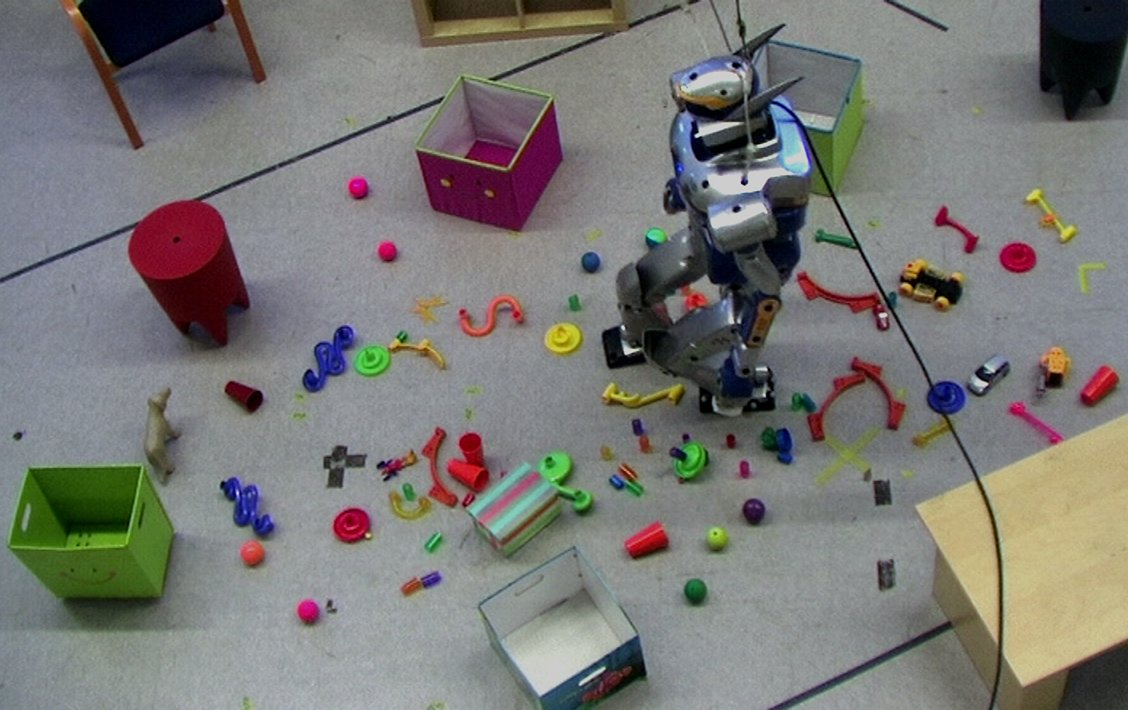
\includegraphics[width=\linewidth]{fig/demo.jpg}}{vid/demo.mp4}
\end{frame}

\begin{frame}{Experimental results}
  \begin{columns}[c]
    \begin{column}{0.5\textwidth}
      \begin{itemize}
      \item Localization uses a motion capture system.
      \item High precision achieved\\
        Error is about 2/3 cm.\\
      \item Correction is computationally inexpensive, run in
        real-time.
      \end{itemize}
    \end{column}

    \begin{column}{0.5\textwidth}
      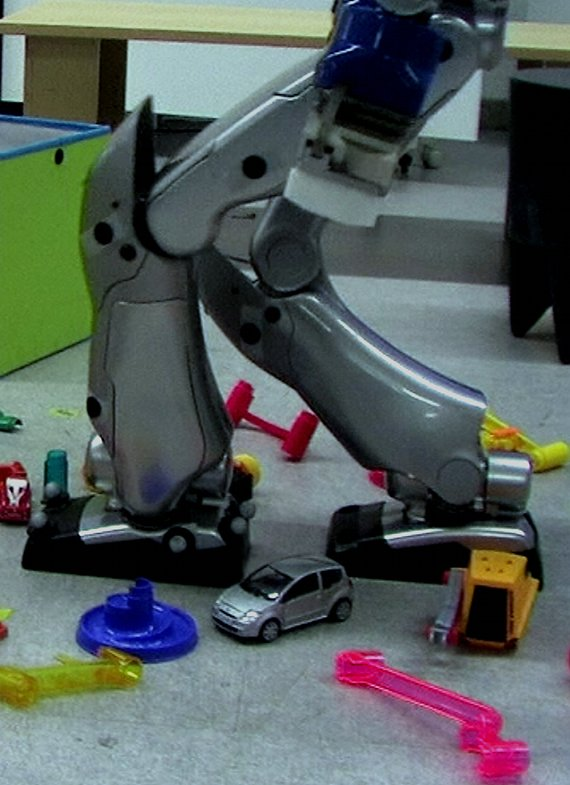
\includegraphics[width=0.9\linewidth]{fig/exp2.jpg}
    \end{column}
  \end{columns}
\end{frame}

\begin{frame}{Future work}
  \begin{itemize}
    \item Online autocollision validation.\\
      {
        \footnotesize
        \cite{10icra.perrin}
      }
    \item Use the embedded vision system to track the robot position.
    \item Allow complex plans execution such as opening a door,
      walking and grabbing an object \ldots

  \end{itemize}
\end{frame}


\end{document}



%%% Local Variables:
%%% ispell-local-dictionary: "american"
%%% End:

%%% 11humanoids-tmoulard-slides.tex ends here
